
%% bare_jrnl.tex
%% V1.4b
%% 2015/08/26
%% by Michael Shell
%% see http://www.michaelshell.org/
%% for current contact information.
%%
%% This is a skeleton file demonstrating the use of IEEEtran.cls
%% (requires IEEEtran.cls version 1.8b or later) with an IEEE
%% journal paper.
%%


\documentclass[letterpaper, 10pt, conference]{ieeeconf}

\IEEEoverridecommandlockouts

\overrideIEEEmargins

\usepackage{graphics} % for pdf, bitmapped graphics files
\usepackage{epsfig} % for postscript graphics files
\usepackage{mathptmx} % assumes new font selection scheme installed
\usepackage{times} % assumes new font selection scheme installed
\usepackage{amsmath} % assumes amsmath package installed
\usepackage{amssymb}  % assumes amsmath package installed
%\usepackage{amsthm}
\usepackage{bm}
\usepackage{mathrsfs}
\usepackage{xcolor}
\usepackage{cite}
\usepackage{threeparttable}
\usepackage{multirow}
\usepackage{bigdelim}
\usepackage{algorithm}
\usepackage{algorithmicx}
\usepackage{algpseudocode}
\usepackage{graphicx}
\usepackage{subfigure}
\usepackage{comment}
\usepackage{array}
\usepackage{hyperref}
\usepackage{galois}
\usepackage{newtxmath}


% correct bad hyphenation here
\hyphenation{op-tical net-works semi-conduc-tor}


\begin{document}
%
% paper title
% Titles are generally capitalized except for words such as a, an, and, as,
% at, but, by, for, in, nor, of, on, or, the, to and up, which are usually
% not capitalized unless they are the first or last word of the title.
% Linebreaks \\ can be used within to get better formatting as desired.
% Do not put math or special symbols in the title.
\title{\LARGE \bf Optimal Object Placement for Minimum Discontinuity Non-revisiting Coverage Task}
%
%
% author names and IEEE memberships
% note positions of commas and nonbreaking spaces ( ~ ) LaTeX will not break
% a structure at a ~ so this keeps an author's name from being broken across
% two lines.
% use \thanks{} to gain access to the first footnote area
% a separate \thanks must be used for each paragraph as LaTeX2e's \thanks
% was not built to handle multiple paragraphs
%

%\author{Michael~Shell,~\IEEEmembership{Member,~IEEE,}
%        John~Doe,~\IEEEmembership{Fellow,~OSA,}
%        and~Jane~Doe,~\IEEEmembership{Life~Fellow,~IEEE}% <-this % stops a space
%\thanks{M. Shell was with the Department
%of Electrical and Computer Engineering, Georgia Institute of Technology, Atlanta,
%GA, 30332 USA e-mail: (see http://www.michaelshell.org/contact.html).}% <-this % stops a space
%\thanks{J. Doe and J. Doe are with Anonymous University.}% <-this % stops a space
%\thanks{Manuscript received April 19, 2005; revised August 26, 2015.}}

\author{Tong Yang$^{1*}$~\IEEEmembership{Student Member,~IEEE}, Jaime Valls Miro$^2$~\IEEEmembership{Member,~IEEE}, \\Yue Wang$^{1}$~\IEEEmembership{Member,~IEEE} and Rong Xiong$^1$~\IEEEmembership{Member,~IEEE}
\thanks{$^1$ Tong Yang, Yue Wang and Rong Xiong are with the State Key 
Laboratory of Industrial Control and Technology, Zhejiang University, P.R. China. 
%Yue Wang is the corresponding author {\tt\small wangyue@iipc.zju.edu.cn}. Rong Xiong is the co-corresponding author {\tt\small rxiong@zju.edu.cn}.
}
\thanks{$^2$ Jaime Valls Miro is with the Robotis Institue at the University of Technology Sydney (UTS:RI), Sydney, Australia.}
\thanks{This work was partially supported by National Key R\&D Program of China (2018AAA0102700), and in part by the Science and Technology project of Zhejiang Province (Grant No.2019C01043).}
\thanks{$^*$ Corresponding author: {\tt\small tong.yang@zju.edu.cn}}
}

% note the % following the last \IEEEmembership and also \thanks - 
% these prevent an unwanted space from occurring between the last author name
% and the end of the author line. i.e., if you had this:
% 
% \author{....lastname \thanks{...} \thanks{...} }
%                     ^------------^------------^----Do not want these spaces!
%
% a space would be appended to the last name and could cause every name on that
% line to be shifted left slightly. This is one of those "LaTeX things". For
% instance, "\textbf{A} \textbf{B}" will typeset as "A B" not "AB". To get
% "AB" then you have to do: "\textbf{A}\textbf{B}"
% \thanks is no different in this regard, so shield the last } of each \thanks
% that ends a line with a % and do not let a space in before the next \thanks.
% Spaces after \IEEEmembership other than the last one are OK (and needed) as
% you are supposed to have spaces between the names. For what it is worth,
% this is a minor point as most people would not even notice if the said evil
% space somehow managed to creep in.


% The paper headers
%\markboth{This paper is concurrently submitted for TMech and AIM 2020 Presentation}{}
%\markboth{Journal of \LaTeX\ Class Files,~Vol.~14, No.~8, August~2015}%
%{Tong \MakeLowercase{\textit{et al.}}: Cellular Decomposition for Non-repetitive Coverage Task Ensuring Least Discontinuities}
% The only time the second header will appear is for the odd numbered pages
% after the title page when using the twoside option.
% 
% *** Note that you probably will NOT want to include the author's ***
% *** name in the headers of peer review papers.                   ***
% You can use \ifCLASSOPTIONpeerreview for conditional compilation here if
% you desire.


% If you want to put a publisher's ID mark on the page you can do it like
% this:
%\IEEEpubid{0000--0000/00\$00.00~\copyright~2015 IEEE}
% Remember, if you use this you must call \IEEEpubidadjcol in the second
% column for its text to clear the IEEEpubid mark.

% use for special paper notices
%\IEEEspecialpapernotice{(Invited Paper)}


% make the title area
\maketitle

% As a general rule, do not put math, special symbols or citations
% in the abstract or keywords.
\begin{comment}
\begin{abstract}
The non-revisiting coverage task of an object using manipulators has been an important application in industrial environment. As the object to be manipulated becomes more and more complex, very rare can a single manipulator establish satisfactory coverage of the target surface with the object and the manipulator base fixed. To tackle this problem, various solutions were proposed, such as choosing a best relative pose between the manipulator base and the object through optimization, or using multiple manipulators. 
However, given the non-bijective nature of the manipulator kinematic, without explicitly considering the joint-space continuity while constructing the coverage path, a continuous coverage path designed in the task-space may easily be truncated into intermittent segments, between which is a path of the manipulator motion with the end-effector (EE) lifting off the surface. Hence, almost all above mentioned algorithms adapt redundant manipulators (even mobile manipulators) to establish enough capability (continuous reachability on the surface) for arbitrary applying of the conventional coverage path planner in the task-space. 
In this work, we aim to create novel partitioning of the task-space that ensures maximal joint-space continuity for the manipulator. Given finite number of possible positions of the object, we allow the manipulator to cover different parts of the surface in different positions nonrepetitively, and the overall discontinuities of the coverage task is proven to be the minimum. 
The proposed algorithm can generate all optimal partitionings, and we show its performance in simulating results on a 5DoF manipulator. 
\end{abstract}
\end{comment}

\begin{abstract}
This work considers the optimal non-revisiting coverage tasks with a single non-redundant manipulator for the case when the object can be positioned at a predefined set of locations within the workcell. The scenario is often encountered in typical industrial settings, for instance when the object presents itself along a conveyor belt and its surface can not be serviced at a single location - the object being large or complex for that endeavour.
%To tackle this problem, various solutions were proposed, such as choosing a best relative pose between the manipulator base and the object through optimization, or using multiple manipulators. 
Given the non-bijective nature of manipulator kinematics between task  and joint space, without explicit consideration of joint-space continuity during its construction, a continuous coverage path designed in task-space may easily be truncated into intermittent segments where the manipulator needs to adopt a different configuration to continue the task, resulting in manipulator motions where the end-effector will need to lift off the surface, an altogether undesirable characteristic affecting the quality of the final product for smooth operations on objects such as polishing, painting or deburring. 
%Hence, almost all above mentioned algorithms adapt redundant manipulators (even mobile manipulators) to establish enough capability (continuous reachability on the surface) for arbitrary applying of the conventional coverage path planner in the task-space. 
In this work, a novel algorithm to optimally partition the task-space whilst considering the various finite locations where the object may be stationed is proposed that ensures joint-space coverage continuity with minimal lift-offs. 
%Given finite number of possible positions of the object, we allow the manipulator to cover different parts of the surface in different positions nonrepetitively, and the overall discontinuities of the coverage task is proven to be the minimum. 
%The proposed algorithm can generate all optimal partitionings, and we show its performance in simulating results on a 5DoF manipulator. 
Results from the algorithm being challenged to achieve coverage of a number of objects, both in simulation and in real tests with an industrial manipulator, prove the effectiveness of the proposed planner when compared with classical coverage strategies faced with the same problem. % <JVM> NOTE we may cite improvement figures here when we get them perhaps, e.g. ratio of lift-offs, time improvements or % of coverage 
\end{abstract}

% Note that keywords are not normally used for peerreview papers.
%\begin{IEEEkeywords}
%Cellular Decomposition, Non-repetitive Coverage Task, Non-redundant Manipulator
%\end{IEEEkeywords}


\section{Introduction}

% The very first letter is a 2 line initial drop letter followed
% by the rest of the first word in caps.
% 
% form to use if the first word consists of a single letter:
% \IEEEPARstart{A}{demo} file is ....
% 
% form to use if you need the single drop letter followed by
% normal text (unknown if ever used by the IEEE):
% \IEEEPARstart{A}{}demo file is ....
% 
% Some journals put the first two words in caps:
% \IEEEPARstart{T}{his demo} file is ....
% 
% Here we have the typical use of a "T" for an initial drop letter
% and "HIS" in caps to complete the first word.

The task of \textit{non-revisiting coverage path planning} (NCPP) for a static object with a robotic manipulator is often undertaken in the manufacturing industry for polishing~\cite{tian2016polishing}, painting~\cite{li2011painting}, deburring~\cite{xie2016grinding}, abbrasive blasting~\cite{Hassan2018Collaboration} or surface defect inspection~\cite{molina2017defects} tasks. 
Generically referred to as the coverage path planning (CPP) problem~\cite{choset2001coverage}~\cite{galceran2013a}, it is defined by the end-effector (EE) traversing over all the points that define the surface of a given object once.
%\begin{color}{blue}
%Optimality of CPP algorithms mainly focus on metrics such as path length and time to completion.
%Atkar \textit{et al.}~\cite{Atkar2003Towards} optimised the coverage path through chossing optimal starting points. 
%Huang~\cite{huang2001optimal} reduced movement cost by remaining on straight paths as long as possible thus minimising the number of turns. 
%Jimenez \textit{et al.}~\cite{jimenez2007optimal} used a genetic algorithm to achieve optimal coverage. 
%However, for manipulator, this essay advocates avoiding unnecessary path lift-off discontinuities as that decidedly outweighs any other performance metric improvement that may be achieved during the coverage process, e.g. by switching between differing geometric paths such as boustrophedon and spirals as proposed in the works of Hassan and Liu~\cite{hassan2018a}.  
%\end{color}

\begin{figure}[t]
\centering
\subfigure[Four different poses for the object with respect to the manipulator. Neither of them ensures coverage (darker colour) of two corner areas by the manipulator (lighter colour), which remain unreachable at this object location.]{
	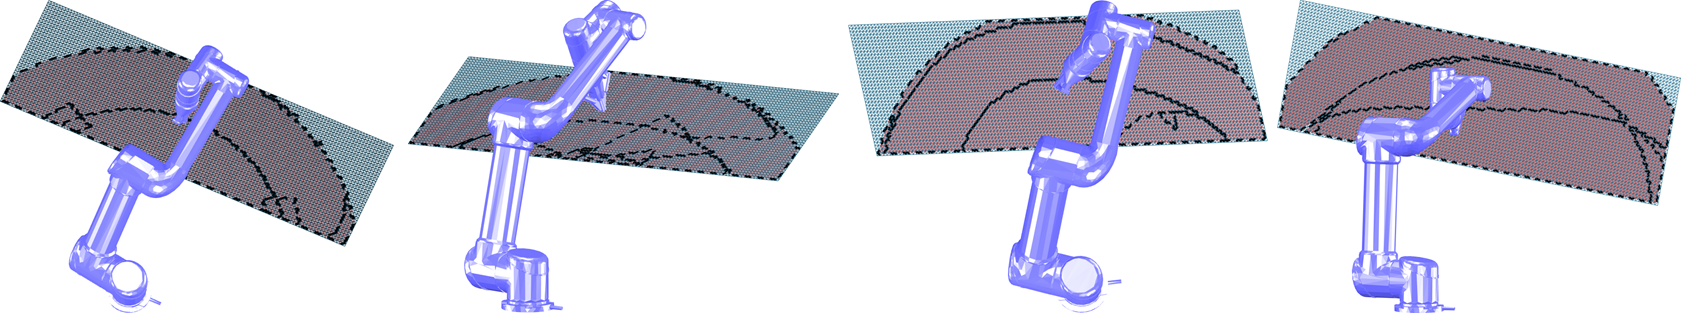
\includegraphics[width = 0.48\textwidth]{figures/planar_demo/fail_comb_2}
	\label{fig:planar:a}
}
%\subfigure[Different IK solutions to reach the same point on the surface. ]{ % <JVM> same orientation in example? unclear
%% <ty> The point is a 2D one, corresponding to a 5D EE pose. This 5 configurations have a same 5D EE pose. 
%	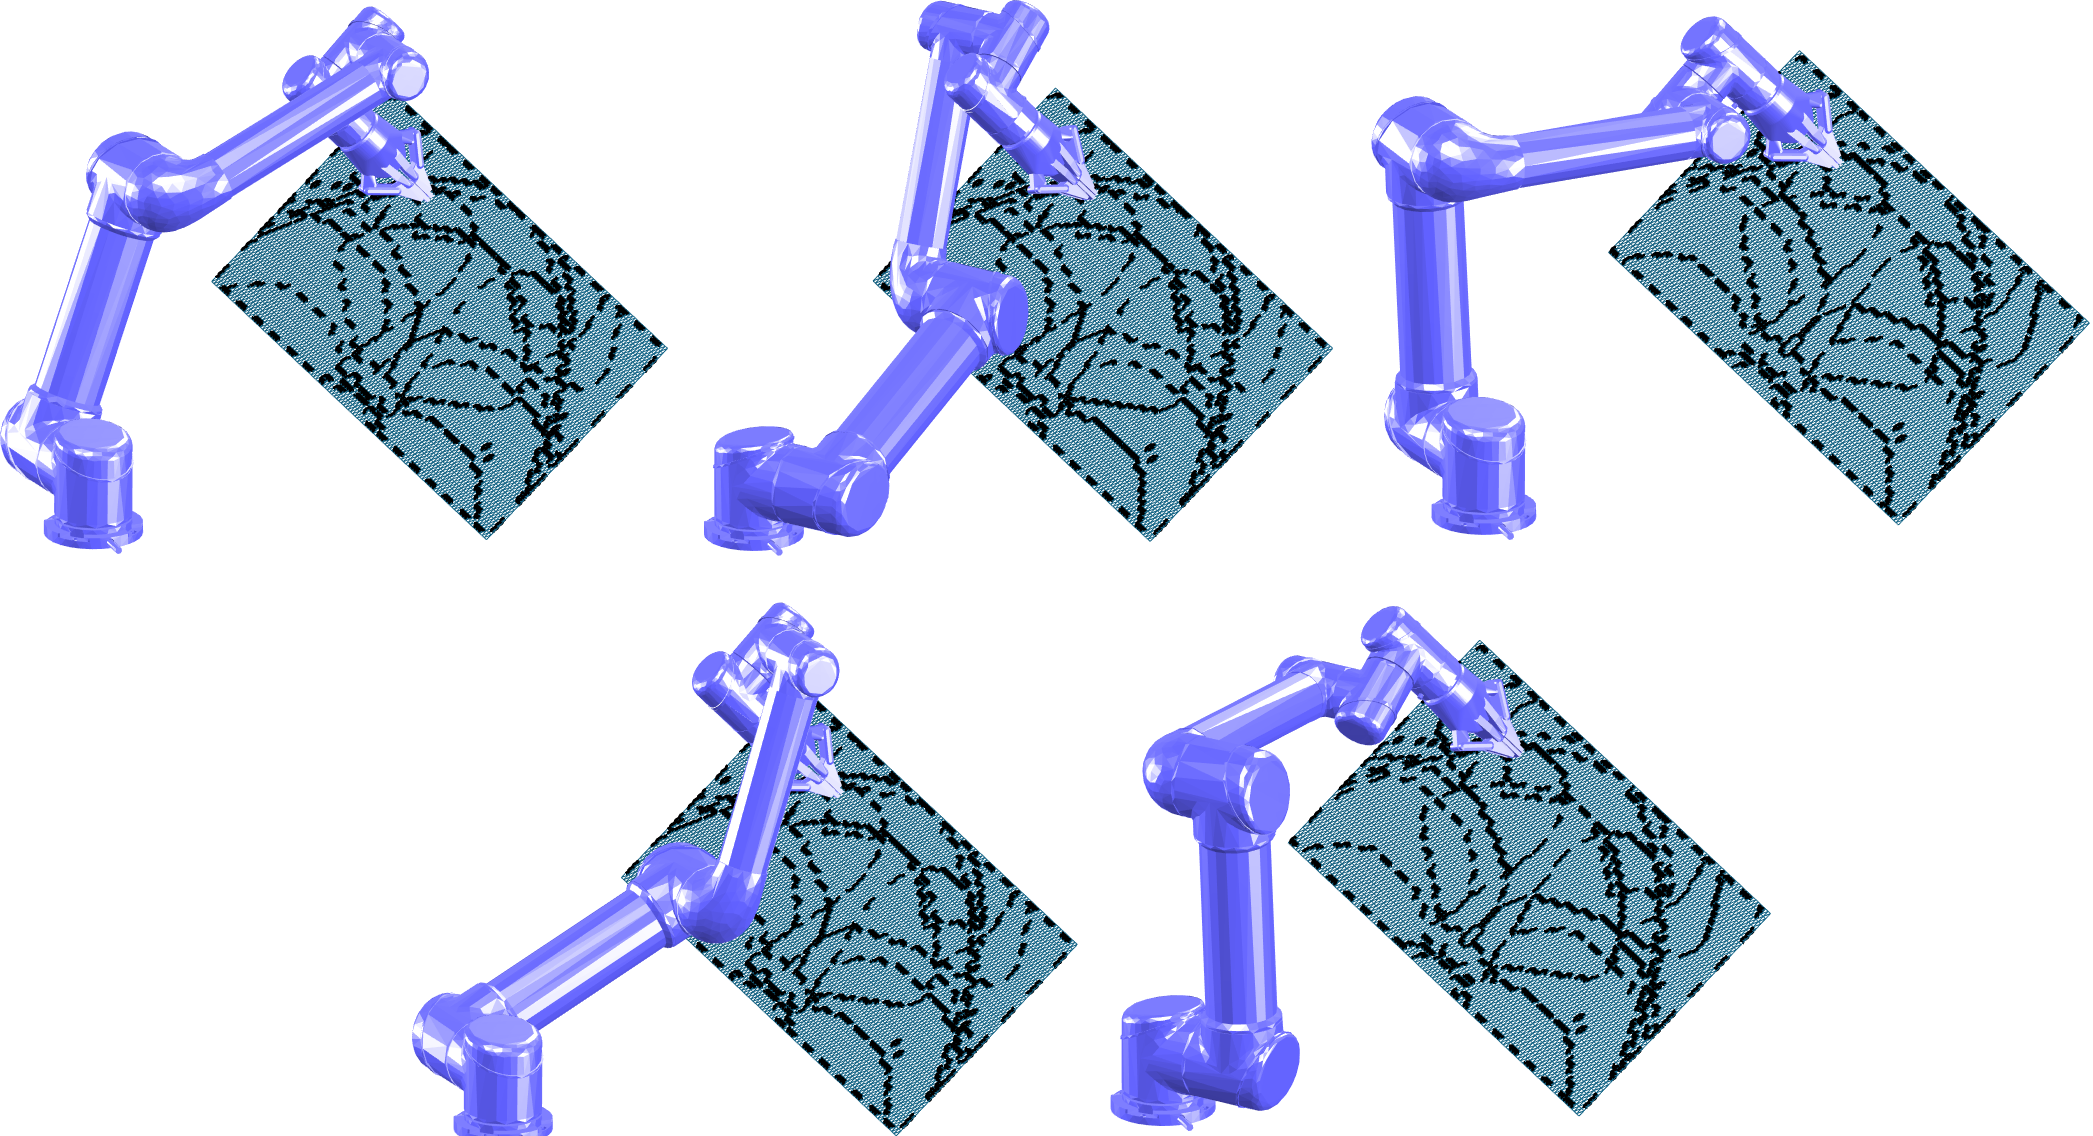
\includegraphics[width = 0.48\textwidth]{figures/planar_demo/demo_comb_2}}
\subfigure[An alternative choice to gain full coverage: first cover half of the object, rotate the object $\pi$ rad. and repeat the process once more on the opposite end. (figures rotated with respect to above to better fit on the page).]{
%	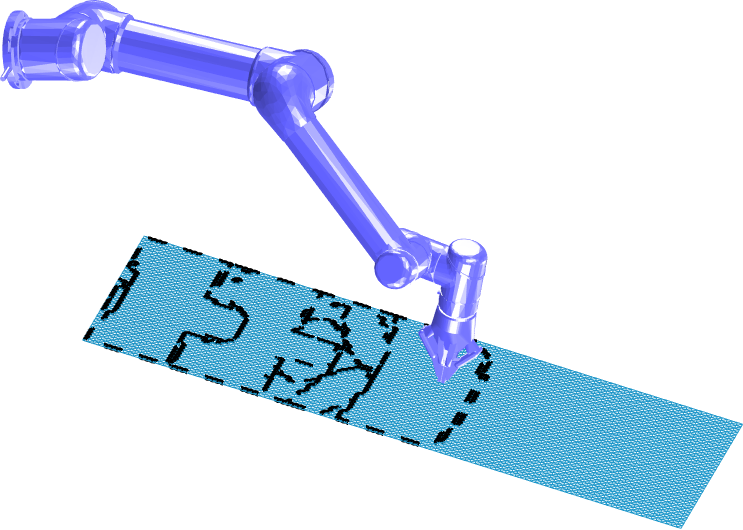
\includegraphics[width = 0.24\textwidth]{figures/planar_demo/alter}
 %  	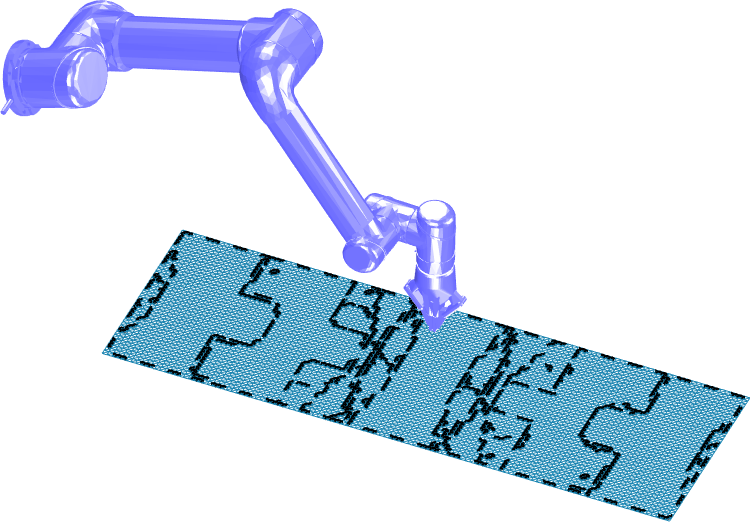
\includegraphics[width = 0.24\textwidth]{figures/planar_demo/alter_complete}\label{fig:planar:b}
  	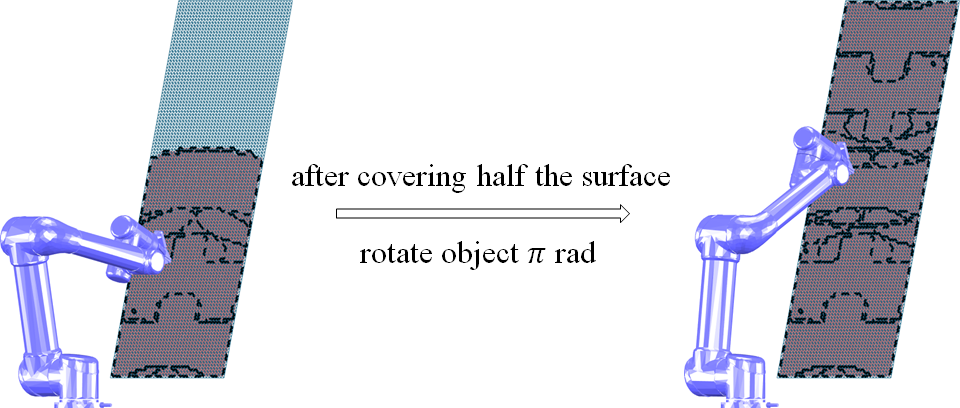
\includegraphics[width = 0.48\textwidth]{figures/planar_demo/alter_comb_3}
	\label{fig:planar:b}
}
\caption{%In (a), a planar object is placed in different poses to find the most suitable pose. In (b) we find a pose for the object that is fully coverable without motion. In many existing literature the full coverage is set as the target, hence this pose is relatively good. However, given such sophisticated distribution of the valid manipulator configurations, if it costs two or more lift-offs to fully cover the object, then it is wiser to alternatively choose another strategy: (c) we only polish half of the surface, and polish the other half after we rotate the object. It has much simpler distribution of valid configurations, and thus is easy to see that the coverage task can be finished within one EE lift-off and one repositioning of the object. 
Illustration of two strategies for full continuous coverage with object replacement: (a) (at least) a single object repositioning and (at least) two EE lift-offs, and (b) using a single object repositioning and requiring only one EE lift-off. The choice of object position drives the associated cell decomposition and the final NCPP and number of EE lift-offs required. 
%2. In fig.1, I think it's better to point out that the black dashed lines refer to the EE trajectories.
%Dashed lines represent the reachable boundary of continuous valid configurations, constructed based on the manipulator IK.
}
\label{fig:planar}
\vspace{-0.5cm}
\end{figure}

Given the non-bijectivity of a manipulator's Inverse Kinematics (IK) when mapping from task to joint space, a continuous section on an object's surface may not be continuously traversable when adopting simplistic greedy strategies~\cite{Yang2020Cellular}. The manipulator will often need to assume alternative configurations to accomplish the coverage assignment, thus incurring suboptimal, often undesirable, and potentially hazardous EE lift-offs. The problem is often compounded by the need to fulfil additional task-specific considerations (e.g. limiting contact forces to pre-specified thresholds, or maintaining a desired EE orientation against the object surface) which further constraint the set of suitable configurations that the manipulator may be allowed to adopt to consummate a coverage task. 

%And it is easy to see from~\cite{Yang2020Cellular} that greedy assignment of the area to be covered cannot ensure optimality. 

For the case when the relative position between the manipulator and the object is known, cellular decomposition strategies have been proposed in the literature dividing free space into simpler regions traversable by conventional coverage paths, generally aimed at guaranteeing minimum overall geometric cost paths~\cite{choset2000exact}~\cite{Acar2002Morse}. 
A globally optimal cellular decomposition algorithm for simple objects has also been proposed to minimise lift-offs by dividing the task-space region into the least number of continuous cells within which the existence of a \textit{joint-space continuous} coverage path can be ensured~\cite{Yang2020Cellular}. The existence of these simply-connected sub-regions then reveals a CPP path between the cells where the number of EE departures from the surface during coverage is optimal. 
% <JVM> this more specific wording can be added to the related work secion instead:
%The algorithm runs iteratively in a deepest-first-searching format, so all optimal physical cellular decompositions can be generated through homeomorphic transformation of the shape of cells. 
The work has been extended to dealing with arbitrary non-simply connected cell topologies, hence allowing more complex forms and task-specific constraints, all whilst guaranteeing an optimal solution in a finite number of steps~\cite{Yang2020Nonrevisiting}.

Given the fixed relative arrangement between manipulator and object, the applicability of these algorithms is however limited by the dimensions of the manipulator workspace, moreover when the object to be manipulated is large or overly complex. The rigid organisation between the pair derives in potentially large surface areas that may remain out of coverage reach. 
The solution to increase reachability with a single manipulator is thus either a mobile manipulator scenario~\cite{Atkar2003Towards} operating around the assembly line and finding appropriate locations to complete the full non-revisiting coverage of the object~\cite{paus2017a}. Or an arrangement whereby the  object may be presented on an assembly line, stopped at certain locations to fully and continuously cover an elected sub-region. Either way, the problem is analogous, allowing the planner increased freedom to position one relative to the other to optimally complete coverage. 
Fig.\ref{fig:planar} illustrates the problem in covering an oversized planar object. Fig.\ref{fig:planar:a} depicts the object at different poses relative to the fixed manipulator base. Neither of them will be able to cover two of the farthest corners of the object in a single go, which calls for (at least one) object repositioning and two EE lift-offs. However, the alternative strategy in Fig.\ref{fig:planar:b} shows two different object poses with respect to the fixed manipulator, where the one on the right depicts a rotation of $\pi$ rad. with respect to the one on the left. With this new arrangement, at each pose half of the surface can be covered, hence full coverage can be achieved with a single object repositioning, and a single EE lift-off. 
Without loss of generality the problem in this paper will be presented assuming a fixed manipulator and a moving object over a finite set of possible poses, the most typical situation in an assembly line. % served by a fixed manipulator.
% <JVM> I leave the multi-manipulator deliberately out as the translation to the specific problem to a multi-arm can lead to another pub

%Then, following a same idea to try different relative poses between the manipulator base and the object, the position of the manipulator base can also vary. That a single manipulator finishes its task in different positions can be analogically adapted into the coverage task carried out by multiple manipulators, where the position of each manipulator is precisely designed to have different reachable area on the surface, and their union covers the whole surface, which is the most commonly used strategy in the realistic assembly line. 
Under this scenario, a point on the surface is coverable as long as it is reachable by at least one of the possible position arrangements for the manipulator-object pair. However, for the NCPP, an area selected to be covered by the manipulator in a previous step cannot be revisited again, resulting in significant restrictions at subsequent covering stages unless planned carefully. The mechanism proposed in this work is able to resolve the optimal group of poses out of a finite set of possible locations for the object in the enlarged operating domain. At each position, part of the surface is manipulated with a singular robot configuration, with the EE then lifting off the surface whilst the object is reposition by stopping the conveyor belt at a chosen pose further along. 
% <ty> we didn't say only one color is allowed for each position. 
EE lift-offs are proven to be the minimum required for optimal coverage. 

The remainder of this paper is organised as follows~\footnote{A video illustrating the concepts hereby described can be found here: \url{https://youtu.be/3ME_IC9ilN0}}.
Section~\ref{sectionrelatedwork} reviews existing literature. 
Section~\ref{sectionproblemformulation} formally defines the problem and the topological graph notation used in the remainder of the manuscript. 
Section~\ref{sectionalgorithm} delves into details to formulate the problem within the NCPP framework. 
Section~\ref{sectiongraphsimplification} describes a strategy to speed-up the solution. Experimental results from simulations and on an actual non-redundant manipulator are collected in Section~\ref{sectionexperiment}, with final concluding remarks gathered in Section~\ref{sectionconclusion}. 


\section{Related Work}
\label{sectionrelatedwork}
When applying conventional \textit{coverage path planning} (CPP) for the manipulator coverage task, reported solutions consist of two stages: first, the target surface is divided into several regions with simple shapes, or cells~\cite{lumelsky1990dynamic}~\cite{choset2000exact}~\cite{Acar2002Morse}. Then, a geometric coverage path, e.g. trapezoidal~\cite{choset2005principles} or boustrophedon~\cite{choset1998coverage}~\cite{choset2000coverage}, are planned on each cell to be tracked by the manipulator EE. 
When faced with coverage tasks for large or complex surfaces, parts of the surface may easily be out of reach and the manipulator cannot establish full coverage. 
%And when the manipulator reaches the marginal region in the work cell, it is ill-conditioned based on some manipulability measure such as~\cite{yoshikawa1990translational}, which is not preferred if we have alternative choices. 

An improvement often proposed in the literature is to choose the best pose for the object, e.g. by formulating the placement problem as a non-linear optimisation problem~\cite{Malhan2019Identifying}. It considers a list of constraints: kinematic reachability, collision avoidance, manipulability, velocity and acceleration limits, etc. 
When a redundant manipulator is assumed, the continuity between two adjacent waypoints in joint-space configuration can be easily judged through the correlation coefficient of their Jacobian matrices~\cite{Chen2002Correlation}. Hence the manipulator coverage task can be completely separated into a two-stage ``CPP-tracking" process. An alternative concept is to employ another manipulator to hold the object, and freely improve the pose when the polishing manipulator finds it difficult to track a pre-defined coverage path on the object~\cite{Kabir2019Generation}. With such high redundancy, the problem is no longer joint-space continuity of the coverage motion, but computational complexity and the presence of local minima in the redundant trajectory planning problem. 
Other methods using non-fixed robot systems with high redundancy have also been  proposed, such as redundant manipulators, dual-arm systems and mobile manipulators~\cite{Atkar2003Towards}. 

When considered from a multiple manipulator system perspective, the area to be covered can be partitioned and assigned to different manipulators. 
Then each robot need not have the ability to operate over the whole object surface, but only focus on its own surface assignment. Strategies include
an area partitioning and allocation by multiobjective optimization and seeding Voronoi graphs~\cite{Hassan2014Task}, combined simulated annealing and genetic algorithm optimisation of the robot base placement~\cite{Hassan2016Modelling}, or a task allocation and optimal number and placement strategy for multi-robot systems~\cite{Kalawoun2018Optimal}, where they fit the problem into the ``Art Gallery Problem''~\cite{Kahn2006Traditional},  which considered the minimum number of guards to visually cover a gallery as a whole. Their proposition combines three commonly used strategies: greedy, genetic, and simulated annealing. 
This is also the case when a single robot (or object) can move to several desired relative poses, whereby at each location part of the surface is covered. Under the assumption that the robot cannot simultaneously do coverage while its mobile base is in motion,~\cite{paus2017a} considered a valid criterion to select the pose of the mobile manipulator. 

It is however noticeable that in all these optimal placement works, the generation of the EE trajectory is independent of the robot, no matter whether they explicitly partition the target surface. 
\begin{comment}
Indeed, some algorithms consider a maximum reaching distance of the manipulator when placing the robot, % <JVM> ideally citation, ideally one we already have
and there has also been a line of work trying generating a capability map for the manipulator. %  <JVM> this needs a citation, "capability of a maniplator" is a very undefinied term. Again, ideally one we already have it!
\end{comment}
%\begin{color}{blue}
Indeed, some algorithms~\cite{Vahrenkamp2013Robot} considered a maximum reaching distance of the manipulator when placing the robot.
~\cite{Zacharias2007Capturing}~\cite{Zacharias2009Using}~\cite{Malhan2019Identifying} tried to pre-compute a discretised representation of the workspace that encodes the position and orientation reachability of the robot. 
%\end{color}
However, the manipulator kinematics is extremely non-linear, and non-bijective (task-joint) within a work cell. Hence any perceived capability cannot be precisely assigned without explicit consideration of the robot inverse kinematics: a coverage path designed without strict assurance of joint-space continuity will easily produce truncated tracing by the manipulator EE, the main concern of the work hereby proposed. 
Noting the inherent joint-space continuity of the Inverse Kinematic (IK) solutions at different points for a given fixed relative pose of the manipulator, object, and the environment, a global optimal cellular decomposition algorithm was proposed, dividing the task-space region into the least number of continuous regions~\cite{Yang2020Cellular}. Within each cell, the existence of a joint-space continuous coverage path could be ensured that guaranteed smooth a provable minimum path truncations. To deal with the non-simply connected topology of cells given more complex task-specific constraints, the work was extended and reformulated as a finite-step algorithm to solve arbitrary topological graphs with multi-connected cells~\cite{Yang2020Nonrevisiting}. 
%The algorithm runs iteratively in a deepest-first-searching format, so all optimal physical cellular decompositions can be generated through a homeomorphic transformation of the shape of cells. 
The solution is hereby further extended to accommodate for a non-fixed scenario, proposing a provable optimal solution to the paradigm.

\section{Optimal Object Placement NCPP}
\label{sectionproblemformulation}
In this section, we first briefly review existing definitions for solving the coverage task with minimum discontinuities, and then solve for the optimal object placement problem. 
\subsubsection{Fixed NCPP Topological Graph Construction}
\label{subsection_NCPP}
The non-revisiting coverage path planning (NCPP) problem was first proposed in~\cite{Yang2020Nonrevisiting}. Here we re-state and adapt some of the notation for the problem at hand. 
Let the non-redundant manipulator base be fixed at the origin. The object (surface) $M$ is placed at $P$ relative to the fixed manipulator base, denoted by $M_P$. The shape of the object $M$, the kinematics of the manipulator $K$, and the surrounding obstacles $\{O\}$ are all known in prior. Point contact between the manipulator EE and the surface of the object is assumed. $\Gamma$ is the set of all paths on $M$. A solution of the coverage task is a set of valid paths $\{\alpha_j\}$ defined on the surface, satisfying: 
\begin{enumerate}
\item Each path corresponds to a set of continuous valid Inverse Kinematic (IK) solutions whose EE covers all waypoints~\cite{Yang2020Nonrevisiting}.  
%The validity of the configuration is given in~\cite{Yang2020Nonrevisiting}.
\label{constraint1} 
\item Paths do not intersect with each other.
\end{enumerate}
Given bijectivity between a set of continuous IK solutions and the surface, colours are used to represent the image of continuous configurations.
% (notwithstanding singular points, where one is arbitrarily chosen). 
Two continuously coverable points on the surface possess the same possible colour. 
Then, following constraint~\ref{constraint1}), a valid path also corresponds to a colour, and it must lie within the coverable area of this colour. 

Let there be $J$ different colours, we can use an indicator function $1_j$ to represent whether we use some of the configurations belonging to the $j$-th set to cover the surface: 
\begin{equation}
1_j =\left\{
\begin{aligned}
&1,\ \mbox{ if there is a path using colour }j\\
&0,\ \mbox{ if there is no path using colour }j 
\end{aligned}
\right., j = 1, \cdots, J
\end{equation}
Then the NCPP problem is to find the optimal set of coverage path segments $\{\alpha_j\}$ such that  
\begin{equation}\label{equ_NCPP}
\{\alpha_j\} = \mathop{{\rm argmin}}\limits_{\{\alpha_j\}\subseteq \Gamma}~\sum\limits_{j = 1}^J 1_j
\end{equation}
Note that $1_j$ will be added twice if there are two paths $\alpha_j, \alpha_{j'}$ that both use the $j$-th configurations. We omit further distinguishment but see them as a whole and denote the NCPP problem by ${\rm NCPP}(K, M_P, \{O\})$. 

\subsubsection{Problem Formulation}
In the optimal object placement problem, the relative poses of the object with respect to the manipulator base is not a single pose $P$ but a finite set of them, denoted by 
\begin{equation}
\{P^i\}, i = 1, \cdots, N, P^i\in SE(3)
\end{equation}
%\begin{color}{blue}
%Without loss of generality, this discrete set of candidate poses is assumed arbitrarily dictated by environmental constraints such as space, collisions, speed of operation, etc. Extending the proposed scheme to a continuous domain is left for future work.
%In general, the initial object placements can be non-trivial, and an experienced engineer can run some sample object placements, and use these as candidates for the algorithm. 
%\end{color}
Once $M$ is located at $P^i$, denoted by $M_{P^i}$, the position of all points to be covered and the surface normal of all points are well-defined, and the set of all paths on $M_{P^i}$ is denoted by $\Gamma_i$. 
The solution of the nonrepetitive coverage path planning problem is to find a set of coverage paths
\begin{equation}
\{\alpha_j^i\}, i = 1, \cdots, N, j = 0, \cdots, J_i 
\end{equation}
where $J_i$ is the number of different colours for the problem ${\rm NCPP}(K, M_{P^i}, \{O\})$, and $\alpha_j^i$ is a curve on the surface $M_{P^i}$ and is executed by the manipulator through the $j_i$-th continuous configurations, such that
\begin{enumerate}
\item Same as~\ref{constraint1}) in Section~\ref{subsection_NCPP}.
\item The concatenation of all paths visit each point on the surface for exactly one time, i.e., \label{constraint2}
\begin{equation}
\bigcup\limits_{i, j} \alpha_j^i = M
\end{equation}
\begin{equation}
\alpha_j^i\cap \alpha_{j'}^{i'} = \varnothing\mbox{ if }i \neq i'\mbox{ or }j \neq j'
\end{equation}
where the union and intersection of paths is calculated in the object's frame. 
\end{enumerate} 
Then, the optimal object placement problem is to find a subset of $\{\alpha^i_j\}$, 
\begin{equation}\label{equ_goal1}
\{\alpha_j^i\} = \mathop{{\rm argmin}}\limits_{\{\alpha_j^i\}\subseteq \bigcup\limits_{i = 1}^N \Gamma_i}~\sum\limits_{i=1}^N\sum\limits_{j = 1}^{J_i} 1_{ij}
\end{equation}
where 
\begin{equation}
1_{ij} = \left\{
\begin{aligned}
&1,\ \mbox{ if a path uses colour }j \mbox{ at position }i\\
&0,\ \mbox{ if no path uses colour }j \mbox{ at position }i 
\end{aligned}
\right.
\end{equation}

Having ensured equation~(\ref{equ_goal1}), a secondary goal can then be established  where we also want the number of object re-positionings to be kept to a minimum, i.e., 
\begin{equation}
\{\alpha_j^i\} = \mathop{{\rm argmin}}\limits_{\{\alpha_j^i\}\subseteq \bigcup\limits_{i = 1}^N \Gamma_i}~\sum\limits_{i=1}^N 1_{i}
\end{equation}
where
\begin{equation}
1_i = \left\{
\begin{aligned}
&1,\ \mbox{ if } &\sum\limits_{j = 1}^{J_i}1_{ij} > 0\\
&0,\ \mbox{ if } &\sum\limits_{j = 1}^{J_i}1_{ij} = 0
\end{aligned}
\right.
\end{equation}
The optimal object placement is clearly a generalisation of the NCPP problem: if $N = 1$ it becomes the NCPP problem. 

\section{Algorithm}
\label{sectionalgorithm}
The main difficulty of the optimal object placement problem is that, say $N = 2$, we can freely divide the surface into two parts, $M^1$ and $M^2$, and let the manipulator cover $M^1$ at $P^1$ and finish $M^2$ at $P^2$. 
Given any divisions of the surface, 
\begin{equation}
M^1\cup M^2 = M,~M^1\cap M^2 = \varnothing
\end{equation}
${\rm NCPP}(K, M^1_{p^1}, \{O\})$ and ${\rm NCPP}(K, M^2_{P^2}, \{O\})$ are fully independent NCPP problems. 

Although a combination of a finite number of NCPP problems is still finitely solvable, there are infinitely many different partitionings to generate $M^1$ and $M^2$. As the problem grows $N = 3, 4, \cdots$, even the initial divisions of the surface cannot be enumerated. 
Hence simply embedding the NCPP solver into the optimal object placement problem is not valid. 
By comparing equation (\ref{equ_goal1}) and equation (\ref{equ_NCPP}), we notice that the optimal object placement problem can be transformed into a NCPP problem as long as the indicator functions with different subscripts can be seen as fully independent numbers. 
This motivates us to consider a generalised object: let $\tilde{M}$ be a virtual object to be manipulated which has $N$ separate parts. 
\begin{equation}
\tilde{M} = \tilde{M}^1\coprod\tilde{M}^2\coprod\cdots\coprod \tilde{M}^N\\
\end{equation}
where the $i-$th part has exactly the same shape as $M$ put at $P^i$, i.e., 
\begin{equation}
\tilde{M}^i \cong M_{P^i}, i = 1, \cdots, N
\end{equation}
and the coproduct sign indicates the non-intersection union of NCPP sub-problems defined in each element, i.e., when calculating the valid configurations for covering $\tilde{M}^i$, any other parts $\tilde{M}^{i'}, i'\neq i$ are not checked in the collision detection module. 
Then, ${\rm NCPP}(K, \tilde{M}, \{O\})$ is finitely solvable, whereby the coverage path covers the original object $N$ times, one time at each position. 
To transform the $N$-time coverage solution to a non-revisiting coverage solution, the most intuitive way is to direct overlap the topological graph of $\tilde{M}^1, \tilde{M}^2, \cdots, \tilde{M}^N$. The definition of this colour in this graph is generalised from a number $j$ to a pair of numbers $(i, j)$. 
Note that the resultant graph does not have physical meaning corresponding to the object being placed at one position, but after solving this graph we will get all optimal combinations within $\bigcup\limits_{i = 1}^N \Gamma_i$. For each solution, the ``colour" not only specifies the inverse kinematic solutions but also corresponds to the position where the object was placed. Finally, now that all optimal solutions of a NCPP problem can be enumerated~\cite{Yang2020Nonrevisiting}, the second goal, minimum number of repositionings for the object, is automatically solved as long as we exhaustively calculate the number for each optimal solution and select the minimal one. 




\begin{figure}[t]
\centering
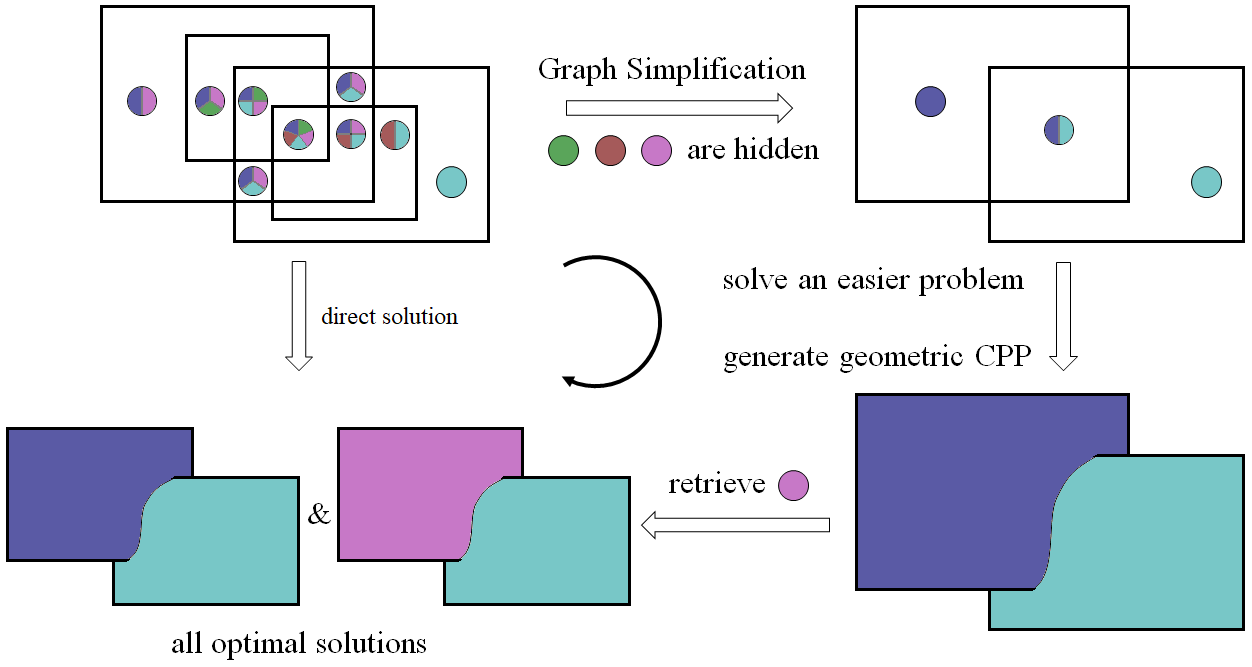
\includegraphics[width = 0.48\textwidth]{figures/graph_simplification}
\caption{Illustration of the graph simplification process, whereby the intial $9$ cells with $5$ different colour configurations are reduced to a graph with $3$ cells and $2$ different colours through prior knowledge of robot kinematics. The ``hidden'' configurations can be reinstated in the optimal solution pool after solving the simplified graph.}
\label{graph_simplification}
\vspace{-0.5cm}
\end{figure}



% <JVM> it would be great to show in a darker blue shade any area that is coverable, as it is not totally clear from graph only. It is clear in Fig 5. I would choose the colour_at_3/color_6 as it shows graph and also the area covered.
\begin{figure*}[t]
\centering
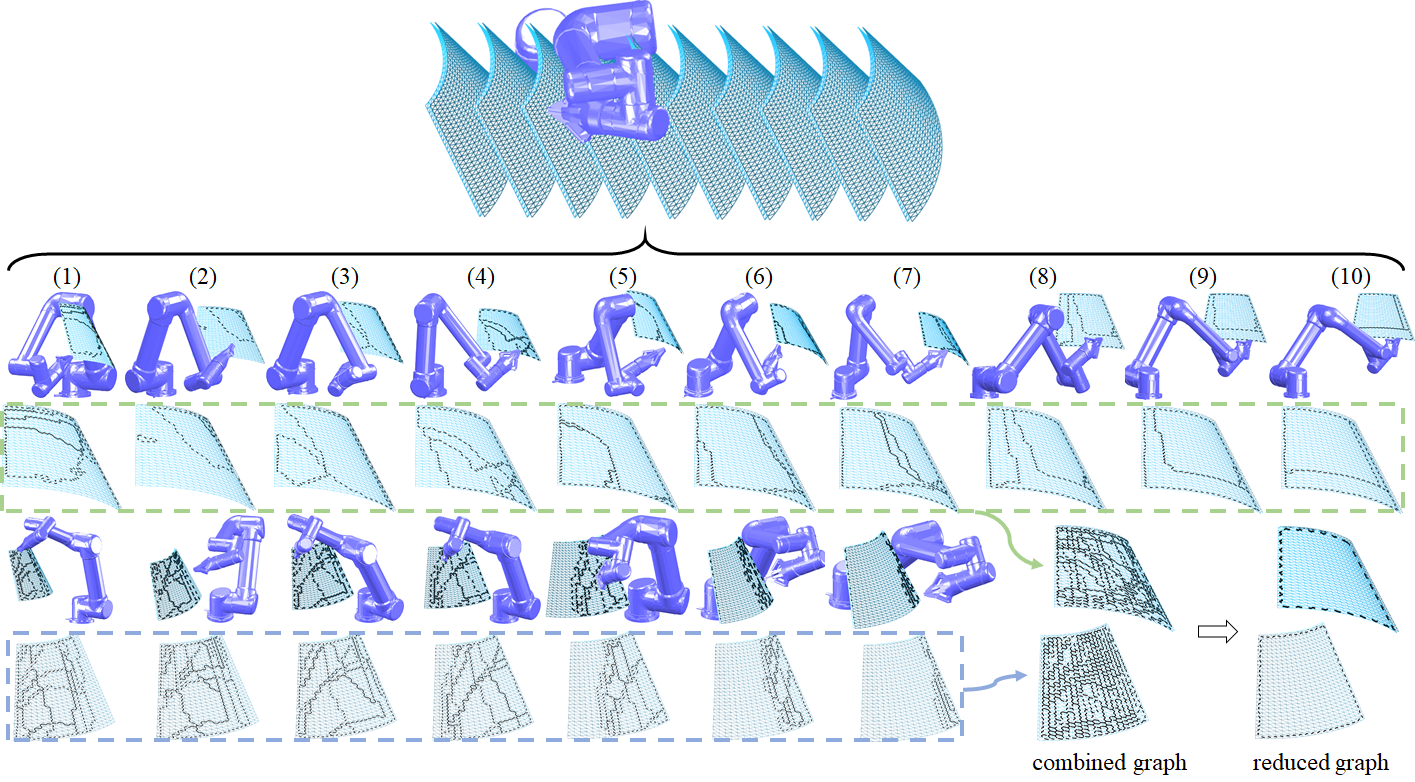
\includegraphics[width = 0.96\textwidth]{figures/blade_demo/whole_process_2}
\caption{Overall representation of the coverage task on a blade-like object at ten discrete equally-spaced locations along a line (station numbers start on the left). None of the ten optional positions can ensure full coverage on both sides of the blade. Specifically, (5)-(10) are capable to complete the concave side (top), whilst only (3) is capable to do so on the convex side (bottom). The convex side is fully uncoverable in (8)-(10) and are not included. We can see that the combined graph, whilst being finitely solvable, quickly becomes overly complex, increasing further with the number of stations being considered. However, the proposed simplification strategy reduces the graph to only two cells, one on each side of the blade's surface. %Then there is even no need for a graph solver. 
}
\label{fig:whole_process}
\vspace{-0.5cm}
\end{figure*}


\section{Graph Simplification for Solver Speed-up}
\label{sectiongraphsimplification}
%computational complexity of the overlapped topological graphs.
As the topological edges from different graphs intersect, each of them is then subdivided into several new edges. The computational complexity will soon blow up as an exponential function of the number of edges. 
It is however noticeable how whilst the focus has been necessarily set on the number of discontinuities, the specific nature of the configurations has been overlooked. 
% <JVM> check my re-wording, make sure it is accurate. I'm a bit concerned that, even if robot is symmetrical, given the relative orientation of robot-object, I would argue you can't assure both cover the same area. Not sure myself about this statement below then ...
% Is there anything else we can assume to discard configurations, other than symetries??
For instance in symmetrical cases, the coverable region of one configuration (e.g. shoulder-left) and another one (e.g. shoulder-right) may be known to be the same, thus so long as we keep in mind that there is an alternative choice (shoulder-right) to cover the same region, we can temporarily ``hide" all shoulder-right configurations and consider only the shoulder-left configurations in the graph. After an optimal physical cellular decomposition has been undertaken, the shoulder-right configurations can be then retrieved and reinserted in the solution pool. 
% <JVM bit of a repetition: because we automatically know that the region assigned to shoulder-left configurations can also be covered with shoulder-right configurations. 
An illustrative example is given in Fig.~\ref{graph_simplification}.

To formally describe the ``hide-retrieve" process, we introduce a partial order set for the colours. 
A partial order set consists of a set together with a binary relation for certain pairs of elements. 
Let $C(i, j)$ be the set of coverable points on the surface using the $j$-th colour when the object is placed at $i$. Then we can create a partial order set $\mathscr{C}$ whose element is $C(i, j), i = 1, \cdots, N, j = 1, \cdots, J_i$, and the partial order is given by 
\begin{equation}
(i, j)\preceq (i', j') ~\mbox{ if }~ C(i, j)\subseteq C(i', j')
\end{equation}
%1. The Section V. is a little bit confusing. How to decide the 'partial order set for the colours'? Is the whole 'graph simplification process' executed manually by the user? Please clarify.
where the comparison between $C(i, j)$ and $C(i', j')$ is the commonplace relation between sets. 
For each comparative sequence of elements in $\mathscr{C}$, we only reserve one upper bound. 
After the geometric cellular decomposition, say a region $C$ is assigned to be covered by the $1$-st colour at position $1$, we have
\begin{equation}
C\subseteq C(1, 1)
\end{equation}
if the comparative sequence in $\mathscr{C}$ is like
\begin{equation}
(1, 2)\preceq (2, 1)\preceq (1, 1)
\end{equation} 
and 
\begin{equation}
C\subseteq C(2, 1),\ C\nsubseteq C(1, 2)
\end{equation}
then we know that this part of the surface can be alternatively covered by using the $1$-st colour at position $2$, but cannot be covered by the $2$-nd colour at position $1$. 

Hiding colours in the graph leads to a reduction in the possible colours for the cells, and can potentially remove edges: it is effectively a speed-up strategy for solving the graph. The simplification strategy can be perceived as aligned with a greedy scheme: the user cannot have a global view on the minimum number of discontinuities for the whole coverage task, but he can always find a pose for the object where he believes a large section of its surface can be covered without discontinuities. Intuitively this means that he provides a relatively large element in the partial order set and is more likely to ``hide" other colours, a perception proven by the blade example.
% <JVM> there seems to be a fair bit of subjectivity - too much "likely" for my like :-) - in these exaplanation. I don't fully understand, so I try and get it when we have more time!!
% <JVM> I will read your other comment in email. I think we should be more scientific than this. Maybe when we do the ball we see whether this also holds, as blade has two different surfaces which is great to prove the intuition, maybe less intuitive on other objects


\section{Experimental Results}
\label{sectionexperiment}

\begin{comment}
\begin{table}[tb]
\centering
\caption{UR5 Manipulator Kinematic Parameters}
\begin{tabular}{|>{ \bfseries }c | c | c | c | c |}
\hline
\normalfont{Joint i}   &     $\bm{\alpha_i}$ [rad]    &   $\bm{a_i}$  [m]    &    $\bm{\theta_i }$ [rad]   &    $\bm{d_i}$  [m]   \\
\hline
\hline
1 & $\pi/2$ & 0 & $\theta_1$ & 0.089 \\
\hline
2 & 0 & $-0.425$ & $\theta_2$ & 0 \\
\hline
3 & 0 & $-0.39225$ & $\theta_3$ & 0 \\
\hline
4 & $\pi/2$ & $0$ & $\theta_4$ & 0.11 \\
\hline
5 & $-\pi/2$ & 0 & $\theta_5$ & 0.09 \\
\hline
EE & $0$ & 0 & - & 0.32\\
\hline 
\end{tabular}
\label{table:ur5_kinematics}
\end{table}
\end{comment}


\begin{table*}[t]
\centering
\caption{Coverage Planners Comparison}
\renewcommand{\arraystretch}{1.2}
\resizebox{\textwidth}{15mm}{
\begin{tabular}{|c|c|c|c|c|c|c|c|c|c|c|c|c|}
\hline
& \multicolumn{2}{c|}{\textbf{Ours} } & \multicolumn{4}{c|}{Fixed pose NCPP~\cite{Yang2020Cellular}} & \multicolumn{2}{c|}{Pure Spiral (10 average)} & \multicolumn{4}{c|}{Pure Boust. (10 average)}\\
\cline{2-13}
& & & \multicolumn{2}{c|}{at (3)} & \multicolumn{2}{c|}{at(5)} & at (3) & at (5) & \multicolumn{2}{c|}{at (3)} & \multicolumn{2}{c|}{at (5)}\\
\cline{4-7}\cline{10-13}
&Spiral&Boust.& Spiral & Boust. & Spiral & Boust. &&& Horizon & Vertical & Horizon & Vertical\\
\hline
\hline
Lift-offs & \textbf{0} & \textbf{0} & 1 & 1 & 1 & 1 & 16.5 & 11.4 & 6.9 & 2.7 & 10.9 & 7.4\\
\hline
Time & \textbf{348.25} & 513.57 & 469.41 & 854.88 & 415.47 &763.82&982.87 & 1026.86 & 989.72& 461.7 & 1174.29 & 709.74\\
\hline
Full Coverage & \textbf{Yes} &\textbf{Yes} & No &No &No &No &No &No &No &No &No &No \\
\hline
\% of coverage & \textbf{100\%} & \textbf{100\%} & 91.46\% & 91.46\% & 82.92\% & 82.92\%& 91.46\% & 82.92\% & 91.46\% & 91.46\% & 82.92\% & 82.92\%\\
\hline
\end{tabular}
\label{table:comparative_results}
}
\begin{tablenotes}
\item $^1$ To make it equitable, the necessary lift-off during transitions between different sides of the object for any of the algorithms are not accounted for.
%\item $^2$ The estimated time is restricted that of actual covering the reachable area. % <JVM> I feel this is obvious
\end{tablenotes}
\vspace{-0.5cm}
\end{table*}


The proposed algorithm selects the optimal set of object positions among a given finite set of possible poses. 
In this section, we imitate the motion of a conveyor belt equipped next to a manipulator, and $10$ possible positions as options for the object to stop and be operated on. 
The simulated and realistic experiments are implemented using a typical 6 DoF manipulator, 
the Universal Robots UR5. % The kinematics of the 6 DoF manipulator are collected in Table~\ref{table:ur5_kinematics}.
For such endeavour, the (commonplace) final revolute joint of the manipulator%~\footnote{\url{https://universal-robots.com/articles/ur/denavit-hartenberg-parameters/}} 
is unnecessary given the rotating nature of the polishing tool itself. 

\begin{figure}[t]
\centering
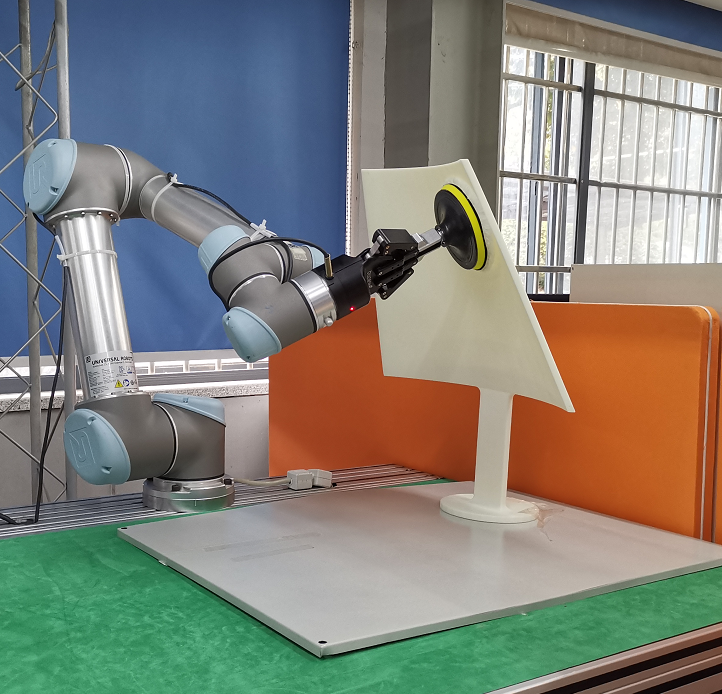
\includegraphics[width = 0.23\textwidth]{figures/real_world/concave_blade_2}
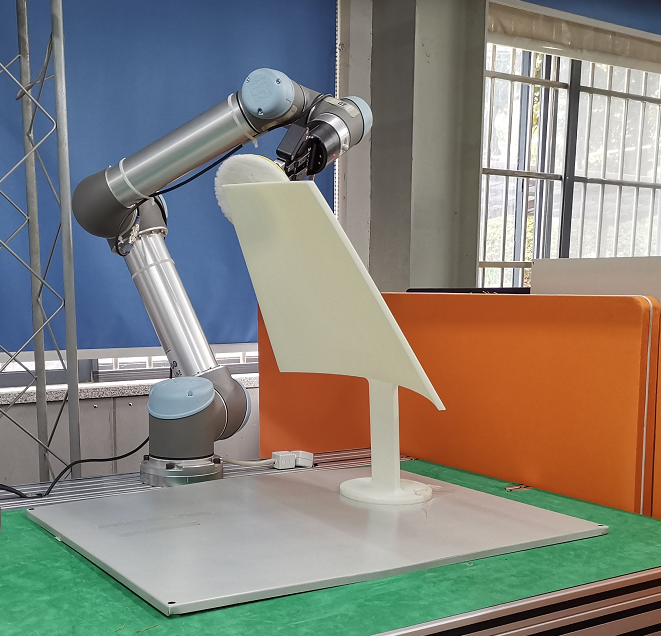
\includegraphics[width = 0.23\textwidth]{figures/real_world/convex_blade_2}
\caption{Example configurations to cover the blade's concave and convex sides. }
\label{fig:real_world}
\vspace{-0.5cm}
\end{figure}


The object employed to illustrate the algorithm is a blade-like curved piece, seen in Fig.~\ref{fig:real_world}, particularly fitting since covering both sides of the blade provides a natural partition of the surface into a convex and a concave side, thus the most suitable positions for covering each side are easily verifiable. 
%Although the blade only bends a little, the orientation of its surface normal varies hugely. 
The reader is referred to the video accompanying the submission where a more detailed visual description of the setup and comparative results are provided, alongside further examples with other objects. 
% <JVM> when you say 'workcell' you mean the rim of the blade, i.e., the thin thickness section around the object? or you mean the working envelope of the robot? I think you mean the former, but 3-3 does not fully show that in my view actually ...
A short polishing tool has been fitted to the EE of the manipulator, making the problem slightly more challenging since on transitioning to the convex side the wrist has to approach the boundary of the work cell where the elbow is almost straight, as seen in Fig.~\ref{fig:whole_process} (3).
% <JVM we don't consider time here, so I don't get this comment: 
%Thus there is only a small window on the conveyor belt for the manipulator to fully cover the convex side. 

The proposed algorithm has been set against comparable fixed CPP alternatives at set locations. Stations 3 and 5 were selected to report results on as being fully reachable within the workspace whilst also offering ample maneuverability in general, hence assumed representative alternatives to operate in a typical workcell unit. 
%Other stations are also compared in the attached video. 
The comparisons include optimally covering the object at a fixed pose~\cite{Yang2020Cellular} and pure template coverage paths (with a Spiral and Boustrophedon paths). Analysis from the proposed object placement NCPP  algorithm with minimal discontinuities is summarised in Table~\ref{table:comparative_results}, where the advancements of the proposed strategy are clearly apparent in regards to guaranteed minimum number of lift-offs, maximum surface coverage, and minimum coverage time. 
It can be seen how only at station (3) full coverage of the convex side can be established. On the concave side, 
%the marginal region of the blade 
%may collide with the upper-arm or fore-arm of the manipulator. Thus the concave side can be fully covered only when the concave side has already been facing the manipulator, (5)$\sim$(10) in Fig.\ref{fig:whole_process}.
stations (5)$\sim$(10) can achieve full coverage, although the movement is constrained to the manipulator already facing the concave side, since any other transition from the convex side will likely induce a collision between the rim and the actual upper- or fore-arm of the manipulator at the desired EE orientations.
%, the marginal region of the blade 
%may collide with the upper-arm or fore-arm of the manipulator. Thus the concave side can be fully covered only when the concave side has already been facing the manipulator, (5)$\sim$(10) in Fig.\ref{fig:whole_process}.


To reveal the performance of the graph simplification strategy, we take the convex side as an example. Since a colour covering the convex side exists at pose (3), it hides all other colours. Thus the simplified topological graph has only one cell with one possible colour. It is so simple that there is even no need for a graph solver. 
On the concave side, a fully-covering colour also exists but the solution is not unique. which means that after solving the one-cell graph, instead of the reserved colour, other colours ensuring full coverage can thus be retrieved. And each of them, together with the unique solution of the convex side, forms an optimal solution to the overall object coverage problem. A more detailed description about the possible colours and solutions is collected in Fig.~\ref{fig:detailed_colour}. 

%The extensive benefits of the proposed algorithm when compared with the other classic techniques in relation to number of lift-offs,  overall execution times to complete the coverage task, and actual achieve coveraged are clearly apparent. 
A detail of the real-world implementation of the optimal coverage task with a 3D print of the same object is shown in Fig.~\ref{fig:real_world}, with more extensive demonstrations reported in the associated video. 


\begin{figure}[t]
\centering
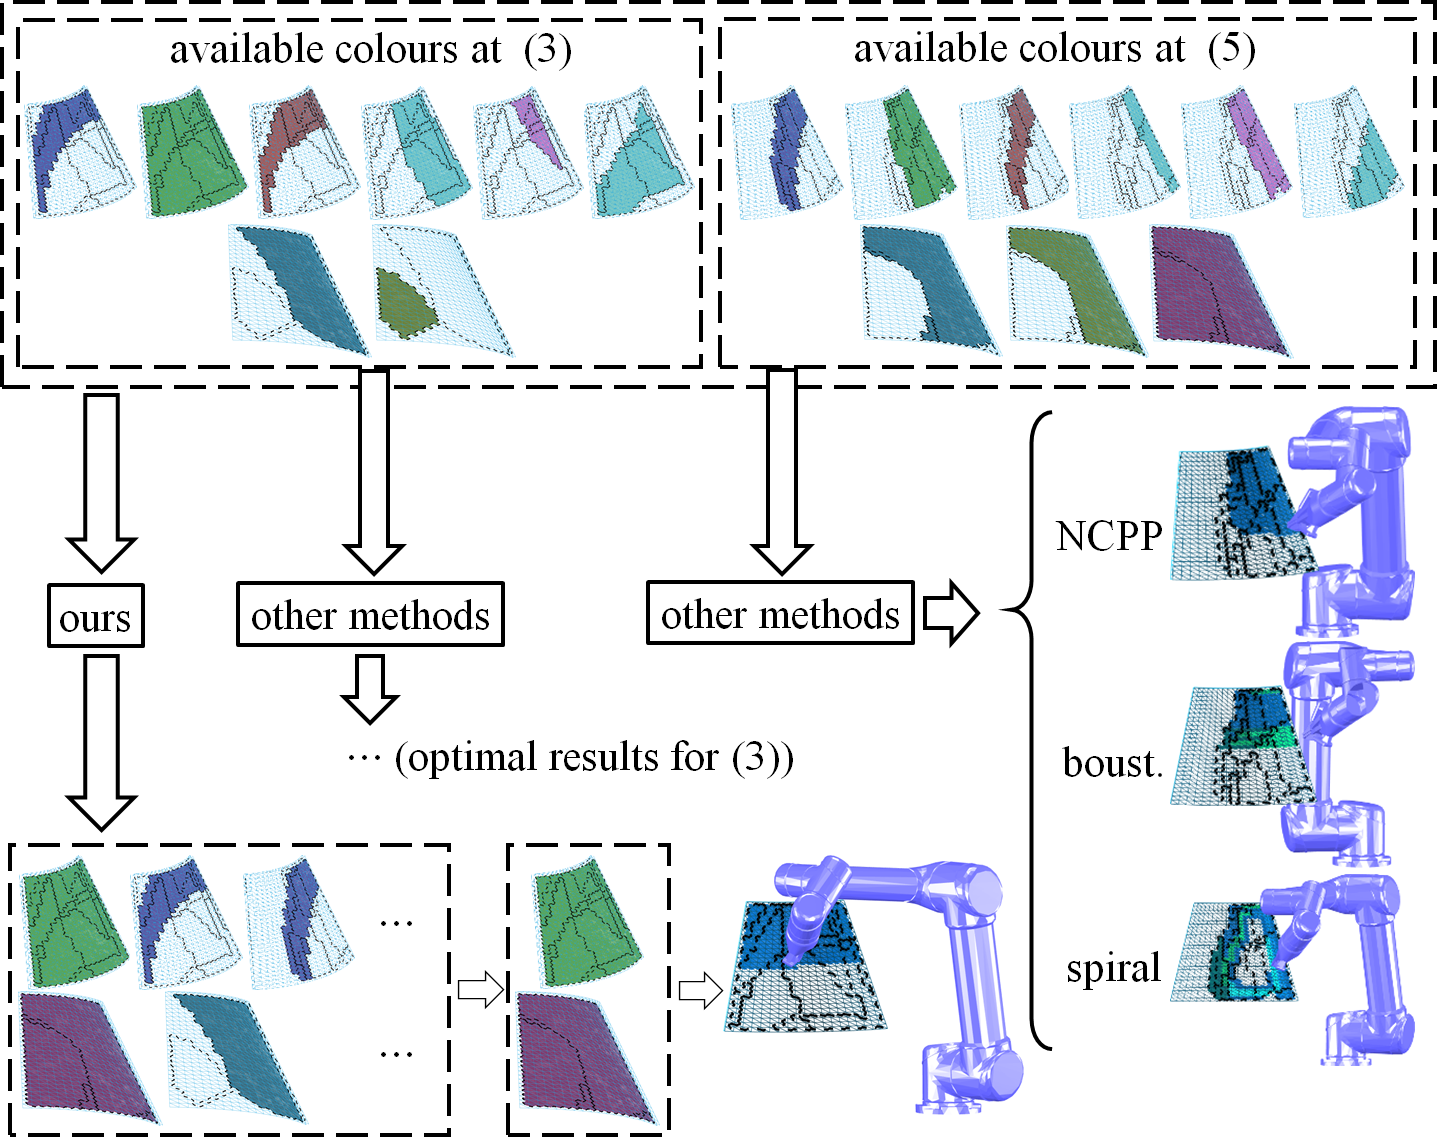
\includegraphics[width = 0.46\textwidth]{figures/blade_demo/details} % <JVM> we have a higher res, details_2, but final pdf is too large. We use "details" - maybe for consideration in final if accepted
\caption{Details of the simulated experiments are shown in Table~\ref{table:comparative_results} on stations (3) and (5). 
%Examples of other CPP solutions are also provided for illustration purposes.
The optimal ($0$ lift-off) solution exists when the object is placed at (3) and (5) for coverage of the convex and concave side, respectively. Regarding the problem as independent NCPP problems at stations (3) and (5) will not achieve an optimal solution, with a requirement for one lift-off on the concave side at (3), and another one on the convex side at (5). And substantially more for non-optimal geometric solutions such as Spiral or Boustrophedon coverage paths.}
\label{fig:detailed_colour}
\vspace{-0.5cm}
\end{figure}

\section{Conclusions}
\label{sectionconclusion}
A novel extension to the NCPP problem formulated with explicit consideration of the coverage task executed at a set of possible object poses has been developed in this work. 
The aim is to minimize the overall number of path discontinuities.%  by planning for the coverage of different parts of the surface at a choice of suitable poses. % <JVM> Note: next paper, continous space!!!
The application is predicated on a typical manufacturing scenario for robotic surface preparation undertaken over a finite set of locations in an assembly line. The proposed scheme leads almost invariably to substantial task execution speed-ups over classical coverage path alternatives.%, as shown in the examples presented.
%Without loss of generality, the problem is extendable to a mobile manipulation unit operating at a set of possible locations in the workfloor. 
By overlapping graphs and solving the combined graphs, all optimal task partitionings are proven finitely solvable. 
After applying any conventional CPP algorithm in each of the resulting cells, the nominated optimal object placement NCPP algorithm is shown able to generate a coverage path containing the provable least number of discontinuities. A comprehensive comparison with other geometric CPPs with a 5 DoF manipulator shows the merit of the scheme and proves the validity of the proposed strategy in producing highly effective coverage paths in a simulated assembly line.
Extensive simulation and real-world implementations in realistic conditions are presented, supplemented by a detailed video illustrating the operation of the algorithm on additional objects. 

\newpage

\bibliographystyle{ieeetr} 
\bibliography{IEEEabrv,ICRA21}


%% You can push biographies down or up by placing
%% a \vfill before or after them. The appropriate
%% use of \vfill depends on what kind of text is
%% on the last page and whether or not the columns
%% are being equalized.
%
%\vfill

% Can be used to pull up biographies so that the bottom of the last one
% is flush with the other column.
%\enlargethispage{-5in}

% that's all folks
\end{document}


